\documentclass[letterpaper,12pt]{article}
\usepackage[parfill]{parskip} % Remove paragraph indentation
\usepackage{amsmath}
\usepackage{float}
\usepackage[margin=1in]{geometry}
\usepackage{graphicx}
\usepackage{placeins}
\usepackage{siunitx}
\usepackage[title]{appendix}
\usepackage{pdflscape}
\usepackage{tabularx}
\usepackage{times}
\usepackage{url}
\usepackage{setspace}
\usepackage[none]{hyphenat}
\usepackage{pdfpages}
\usepackage{longtable}
\usepackage{tikz}

\DeclareSIUnit{\samplepersec}{SPS}

\begin{document}

\begin{titlepage}
    \begin{center}
        \vspace*{1cm}

        \Large
        \textbf{ELEC 490/498 Project Blueprint Document}

        \vspace{0.5cm}
        Group 18\\
        TeachEE\\
        \vspace{0.5cm}
        \normalsize
        \textbf{John Giorshev (20103586, john.giorshev@queensu.ca) \\ Eric Yang (20120750, e.yang@queensu.ca) \\ Ethan Peterson (20105011, 17emp5@queensu.ca) \\ Timothy Morland (20096286, 17tm22@queensu.ca)}\\
        \vspace{0.5cm}
        Submitted November 22, 2022\\

        \vfill
            
        \textbf{To:}\\
        Instructor Dr. Michael Korenberg (korenber@queensu.ca) \\
        Instructor Dr. Alireza Bakhshai (alireza.bakhshai@queensu.ca) \\
        Instructor Dr. Alex Tait (alex.tait@queensu.ca) \\
        Instructor and Supervisor Dr. Sean Whitehall (sw109@queensu.ca) \\
        Supervisor Dr. Thomas Dean (tom.dean@queensu.ca) \\
            
        \vspace{1.8cm}

    \end{center}
\end{titlepage}
\setstretch{1.5}
\pagenumbering{gobble}
\section*{Executive Summary}

This report outlines TeachEE, a device which facilitates online learning for
electrical engineering labs. It describes the project's scope: a minimum viable
product for the purpose of this capstone project, with room for scope expansion
later in the year if circumstances allow it. The minimum viable product consists
of an oscilloscope, desktop app, and communication between a computer and the
device via USB. A complete list of specifications for the MVP are provided in
Table \ref{hw:specs-table} and Table \ref{sw:specs-table}.

This blueprint also outlines a road map for this project; most hardware related tasks have
been completed, with the software related tasks scheduled for completion later
in the term. Although the PCB shipment from the manufacturer was delayed, the
project is still on schedule. Additionally, for the upcoming tasks, there is a
clear and equal division of responsibility between group members, as shown in
Table \ref{hw:milestones-table}. The project is scheduled to be completed by
week 20, two weeks before the Open House, to allow for extra time in case of
emergencies.
\newpage

\setstretch{1}
\tableofcontents
\listoffigures
\listoftables
\newpage
\setstretch{1.5}
\pagenumbering{arabic}
\section{Introduction} \label{sec:intro} % Ethan
This blueprint outlines Group 18's capstone project TeachEE,
originally proposed in ELEC 390 \cite{prop_390}, and provides the baseline
specifications for TeachEE. These specifications should be treated as guidelines
for the minimum project performance required at the Open House in March. This
report is intended for the ELEC 498 instructors and Group 18's supervisors. It
consists of the methodology of completing the project, progress up to
the time of writing this document, budget, and strategies to mitigate potential
issues. The appendices of this report include technical information that
supplement the report body.

% NOTE: what I had before: (came after remote delivered eng labs)
% At a design level, the device will require
% both a custom Printed Circuit Board, device driver, and graphical user interface
% to function correctly. There are two key technical challenges in this project;
% the Printed Circuit Board (PCB) and device driver software.
\subsection{Design Problem}
TeachEE is a device that acts as a general purpose electronics measurement
instrument for remotely delivered engineering labs. The device acts as both a
USB oscilloscope and current monitor. Currently, there are few instrumentation
options for students completing their labs remotely. TeachEE bundles
together the functionality most commonly required for electrical engineering
labs and packages it with portable software that can run on lower end computers
with any operating system.

The PCB is a large technical undertaking as it must be able to capture both
voltage and current samples at a rate that is useful to undergraduate students.
Moreover, the PCB must contain custom circuitry to relay the sample data over
USB, which requires controlled impedance transmission
lines. Additionally, the PCB will need multiple high speed clocks for
the USB PHY (PHYsical layer chip) and Analog to Digital Converter (ADC). Further challenges include
analog signaling and sufficiently filtering and protecting the inputs.

The second key technical challenge in this project is the device driver for the
oscilloscope. The USB 2.0 link between the device and laptop has a throughput of
up to 480 Mbps. This requires performant driver software that can quickly process
the sample data and relay it to the GUI frontend. The software will also require
a packet framing technique that can efficiently separate current and voltage
samples.

In terms of design changes, the voltage power
sources have been removed and the microcontroller has been changed to an FPGA,
which has been discussed with the team's hardware supervisor.
% Ethan
% Explain the design problem Hardware software timeline
% 275 words max
\subsection{System Specifications} \label{sec:specs}
The following tables outline the target hardware and software specifications of
this project.

% \newcolumntype{b}{X}
% \newcolumntype{s}{>{\hsize=.2\hsize}X}
% \newcolumntype{m}{>{\hsize=.4\hsize}X}
\begin{table}[H]
    \caption{Hardware Specifications}
    \begin{tabularx}{\textwidth}{l|l|l|l}
          & Specification & Target Value & Tolerance \\
        \hline
        1 &Voltage Input Bandwidth&\SI{100}{\kilo\hertz}& $\pm \SI{1}{\kilo\hertz}$ \\
        2 &Current Input Bandwidth&\SI{100}{\kilo\hertz}& $\pm \SI{1}{\kilo\hertz}$ \\
        3 &Measureable Current Range&\SI{-15}{\ampere} to \SI{+15}{\ampere}& $\pm \SI{5}{\ampere}$ \\
        4 &Measureable Voltage Range&\SI{0}{\volt} to \SI{3.3}{\volt}& $\pm \SI{200}{\milli\volt}$ \\
        5 &Number of Current Input Channels& $1$ & $0$ \\ 
        6 &Number of Voltage Input Channels& $1$ & $+2$ \\
        7 &Power Input Voltage Rating& \SI{5}{\volt} & $\pm \SI{500}{\milli\volt}$ \\
        8 &Power Current Consumption Rating& \SI{500}{\milli\ampere} & $\pm \SI{250}{\milli\ampere}$ \\
        9 &Voltage Sample Rate& \SI{1}{\mega\samplepersec} & \SI{0}{\mega\samplepersec}\\
        10 &Current Sample Rate& \SI{1}{\mega\samplepersec} & \SI{0}{\mega\samplepersec} \\
        11 &PCB Thickness& \SI{1.6}{\milli\metre} & $\pm \SI{0.1}{\milli\metre}$ \\
        12 &PCB Dimensions& \SI{0.04}{\meter\squared} & $\pm \SI{400}{\milli\metre\squared}$ \\
        13 &Voltage Sample Error against commercial scope & N/A & $\pm \SI{20}{\percent}$ \\
        14 &Current Sample Error against commercial meter& N/A & $\pm \SI{20}{\percent}$
    \end{tabularx} 
\label{hw:specs-table}
\end{table}

% Timbo / Ethan
\begin{table}[H]
    \caption{Software Specifications}
    \begin{tabularx}{\textwidth}{l|l}
        \textbf{1} & \textbf{Functional Requirements}\\
        \hline
        1.1 & The software shall be able to modify the horizontal and vertical scales of the plot. \\
        1.2 & The software shall be able to modify the trigger voltage. \\
        1.3 & The application shall be deployable to Windows, macOS, and Linux. \\
        \hline
        \textbf{2} & \textbf{Interface Requirements} \\
        \hline
        2.1 & The software shall be able to capture voltage samples and export them to a CSV file. \\
        2.2 & The software shall receive samples via the FTDI 232 in synchronous mode. \\
        \hline
        \textbf{3} & \textbf{Performance Requirements} \\
        \hline
        3.1 & The software shall be able to render waveforms at a rate of \SI{30}{\hertz} on screen.
    \end{tabularx} 
\label{sw:specs-table}
\end{table}

% 1-2 tables (maybe one for HW SW)
% Ethan will write some hardware and software specs here in a table

\section{Methodology} % ERIC
% 1.5 pages max for everything

\subsection{Approach}

% Software
The software aspect of TeachEE will be a desktop application
with a web-based user interface. This reduces costs as the display and
processing power of the user's machine can be used instead of additional
hardware. Exporting voltage and current samples can be done
by saving to a CSV file. The application will be built using
Tauri, a framework that utilizes a Rust binary as a backend and JavaScript,
HTML, and CSS as the frontend.

% Hardware
The TeachEE hardware design will be a standalone PCB and FPGA module with
access to a USB controller and an Analog to Digital Converter (ADC). This FPGA
module will be connected to a socket on the PCB rather than soldered on; since
they are highly complex, this approach will reduce development time and allow
the FPGA to be replaced in the event of a hardware failure. A full hardware
system block diagram is given in Appendix \ref{appendix:block-diagram} below.

\subsection{Design Tools, Hardware, Instrumentation}
Tauri was chosen as the application framework because of its high performance
and low binary size when compared to other Rust frameworks 
\cite{tauri_benchmarks}. As TeachEE is intended for remote use, being
lightweight is important for quick deployment and operation.

The backend will be written in Rust to address the high throughput and
data processing requirements due to its high run time speed \cite{rust_speed}.
Furthermore, Rust provides support for concurrent programming, which may be
necessary to speed up data stream processing. The frontend will be written in
plain JavaScript to avoid the performance overhead of abstractions in
JavaScript frameworks \cite{javascript_speed}. Although modularization can
improve code maintainability, it is not necessary for this project because the
user interface will be relatively simple.

The primary design tool used for the hardware is Altium with the PDN Analyzer
extension. Altium is a full PCB schematic and layout design suite. The software
will also produce fabrication files in a standard format that can be given to
manufacturers. PDN Analyzer provides tools for checking the Power Distribution
Network (PDN) of the PCB. It is used as a final verification that the PCB
traces can carry enough current to supply all the devices on the board.

\subsection{Validation}
Tauri provides Tauri Action, which is a Github Action that builds Tauri
applications into native binaries on Windows, macOS, and Linux
\cite{tauri_actions}. This feature will be used to provide continuous integration
to the project and ensure correctness on all targeted platforms. Additionally, unit
tests can be written for signal processing functions such as Fast Fourier Transform.

The accuracy of TeachEE can be determined by measuring the same signal with both a
commercial oscilloscope and TeachEE.
The degree of accuracy will be indicated by voltage and current differences
given by the target percentages in Table \ref{hw:specs-table} above.

\section{Progress to Date} % Ethan / Tim for HW/SW respectively
Since the start of the term, the team has completed a set of both hardware and
software tasks.
% Explain that there has been a completed hardware design.
% include schematics, layout and BOM in Appendices

\subsection{Hardware Design}
At this time, the initial printed circuit board schematic and
layout are complete. The PCB system block diagram is shown in Appendix
\ref{appendix:block-diagram}. Full schematic and layout prints are supplied
in Appendix \ref{appendix:schematic} and \ref{appendix:layout} respectively.

The block diagram is a simplified version of the schematic and thus does
not enumerate each part on the PCB. A full bill of materials for the PCB can be
found in Appendix \ref{appendix:bom}. The two critical blocks of the diagram are
the USB FIFO and ADC. Voltage samples are fed into TeachEE via the BNC connectors
on the PCB. Two additional voltage channels are added for redundancy purposes,
but the minimum requirement is one channel. Adding additional functionality to
the hardware allows for future software extensibility. The
ADC input going directly to the FPGA is filtered by a Low Pass Filter (LPF) to
prevent aliasing in the frequency domain. The discrete ADC also has an LPF in
addition to a dedicated driver for the differential inputs on the chip. The
driver amplifier protects the ADC against out of bound voltages.

\subsection{Software Design}

At the time of writing, the skeleton for the TeachEE desktop app is complete.
Currently, the app has three main components: USB Manager; Storage;
and Frontend.  The USB Manager and Storage components are
written in Rust and operate as separate threads in the same process; the
USB Manager reads and writes from data in Storage through
thread-safe getter/setter methods. The Frontend component is written in
Javascript and operates in its own process; it communicates with the Storage
component through message passing. JavaScript and Rust interoperability is
enabled by serializing all messages into JavaScript Object Notation
(JSON) strings. The relationship between the above-mentioned components is
summarized in Figure~\ref{sw:architecture}.

\begin{figure}[h]
    \centering
    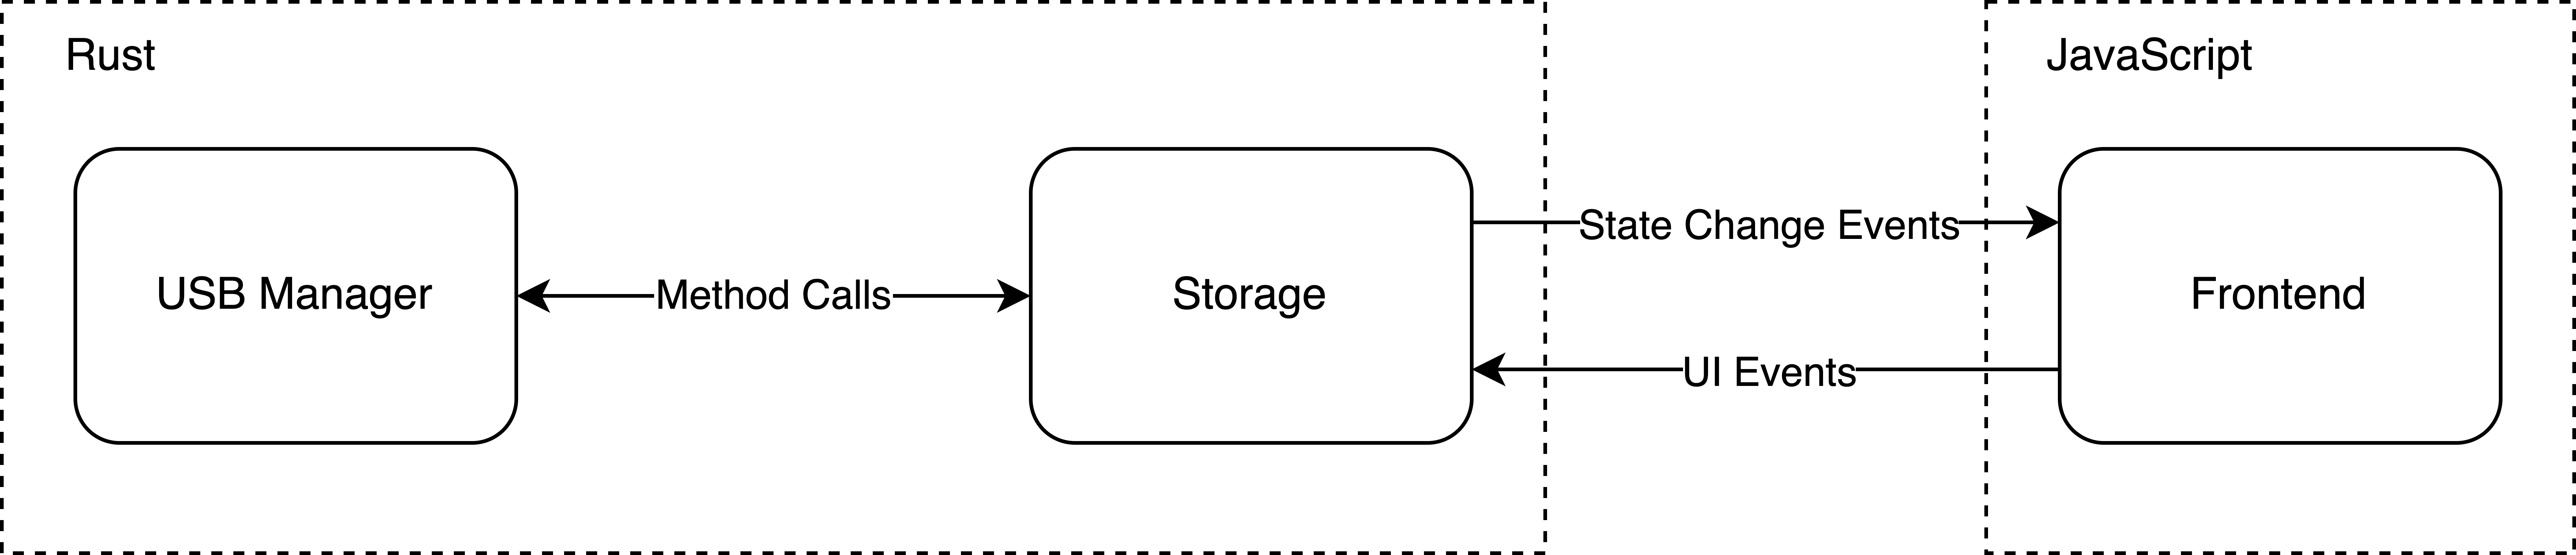
\includegraphics[width=\textwidth]{schematics/sw-architecture.png}
    \caption{TeachEE Desktop App Architecture}
    \label{sw:architecture}
\end{figure}

The performance of this architecture has been validated by displaying artificial
data generated at the same sample rate as the real hardware. At present the app
is able to display waveforms at a frame rate of 60 Hz while consuming an
insignificant amount of system resources on a 2022 M2 MacBook Air. Screenshots
of the app can be found in Appendix~\ref{appendix:screenshot}.

\subsection{Milestones and Division of Labour}
% Table of major and intermediate milestones (ERIC)
% Each table cell should include due date and assigned member
The following table lists the milestones associated with this project and the
team member(s) responsible for each.
\begin{table}[H]
    \caption{Milestones}
    \begin{tabularx}{\textwidth}{l|l|l|l}
        No. & Milestone & Due date & Responsible Member(s) \\
        \hline
        1 & Design and order PCB & Week 4 & Ethan \\
        2 & Create skeleton of application & Week 11 & Tim \\
        3 & Submit blueprint report & Week 11 & All members \\
        4 & Verify PCB is functional & Week 12 & Ethan \\
        5 & Read values from USB driver & Week 13 & Tim and John \\
        6 & Create basic UI and waveform display & Week 14 & Eric \\
        7 & FPGA programming & Week 16 & Ethan \\
        8 & Implement oscilloscope triggering & Week 16 & John \\
        9 & Implement CSV exporting and all UI functionality & Week 17 & Eric \\
        10 & Testing of application & Week 18 & Tim, Eric, and John \\
        11 & Testing of PCB & Week 18 & Ethan \\
        12 & Testing of complete system & Week 20 & All members \\
        13 & Open House & Week 22 & \\
        14 & Final deliverable & Week 23 & \\
        15 & Final project report & Week 24 & All members
    \end{tabularx} 
\label{hw:milestones-table}
\end{table}
\section{Budget} % Ethan
% include some preamble wrt board quantities and BOM table
% consider ActiveBOM from Altium for this.
% BOM probably takes too many pages, will need to attenuate

The budget of 600 dollars provided by the department is sufficient for this
project assuming only one unit of the device is manufactured, nonetheless,
three units have been ordered. However, the team will only submit a reimbursement
request for one unit. The two remaining units will be for personal use only.
Additional electrical instruments, such as oscilloscopes
and signal generators for debugging, are not included in the budget as they will be
accessible on campus.

\subsection{Materials and Supplies}
Table \ref{tab:abbreviated-bom} breaks down the cost of the PCB
fabrication and assembly as quoted by the supplier. The supplier contracted for
TeachEE is Bittele (7PCB). Bittele takes care of both the fabrication and
soldering of the PCBs. Moreover, Bittele takes the generated output from the EDA
software (Altium) and procures all the parts directly to their facility. The
procurement cost is expanded in the budget table with the major functional
components on the PCB. An exhaustive list is not included as there are hundreds
of miscellaneous resistors, capacitors, and inductors whose cost is marginal.

A full unit of the PCB comes in \$80 under budget. This leaves
additional budget to purchase any replacement components or
cover unexpected expenses. Should the project still exceed the budget, the team
will first contact the project supervisors to see if there is a possibility of
additional funding. The full BOM for the PCB is provided in
Appendix \ref{appendix:bom}.

\begin{table}[H]
    \caption{TeachEE Bill of Materials}
    \begin{tabularx}{\textwidth}{l|l|l}
        \textbf{Item / Part Number} & \textbf{Supplier} & \textbf{Cost (CAD)} \\
        \hline
        PCB Fabrication & Bittele & \$104.37\\
        PCB Total BOM Procurement & Bittele & \$126.67\\
        \hline
        \textbf{Major Components (Included in cost above)}& &\\
        \hline
        AD9288BSTZ-40 ADC & Digi-Key & \$14.70\\
        AD8138ARZ-R7 ADC Driver & Digi-Key & \$26.85\\
        FT232HQ-REEL USB FIFO & Digi-Key & \$6.41\\
        ACS720KLATR-15AB-T Current Sensor & Digi-Key & \$9.81\\
        \hline
        PCB Assembly & Bittele & \$289.76\\
        \hline
        Total & & \$520.80\\
        \hline
        Budget Remaining & & \$79.20
    \end{tabularx} 
\label{tab:abbreviated-bom}
\end{table}

\subsection{Contributions From Other Sources}
There are no outside contributions at the time of writing this report. However,
the team will reach out should additional funding be required. 

\section{Potential Problems and Mitigation Strategies}
% Ethan (Make a single table)
There are two main categories for which technical problems can arise in this
project. Issues are likely to come in the PCB design and in the FPGA Real Time
Logic (RTL) code. Software remains less of a concern as compile times are
instantaneous when compared to FPGA synthesis or lead time of a new hardware
revision. Software can still be a source of potential problems, however,
hardware or FPGA failure are of greater severity. Table \ref{tab:issue-mitigation}
summarizes possible issues in the PCB and FPGA along with ways to reduce their
probability or recover from them.

\begin{table}[H]
    \caption{Potential Problems and Mitigation}
    \begin{tabularx}{\textwidth}{p{1.5in}|p{2in}|p{2.5in}}
        \textbf{Problem Description} & \textbf{Possibility Reduction} & \textbf{Course of Recovery} \\
        \hline
        USB FIFO chip on the PCB does not work or the FPGA cannot successfully
        interface with it.
        & Choosing a PCB layout that is suited to the high-speed control signals
        running between the USB-FIFO, ADC and FPGA.
        & Use the built in USB unit on the FPGA module, which supports 12Mbps.
        The slower speed satisfies the required sample rate of
        \SI{1}{\mega\samplepersec} and \SI{100}{\kilo\hertz} bandwidth.\\
        \hline
        Discrete ADC does not work.
        & Following the reference design given in the datasheet and
        installing differential ADC drivers for input protection.
        & Use the built in ADC on the FPGA module. This built-in ADC satisfies the
        \SI{1}{\mega\samplepersec} and \SI{100}{\kilo\hertz} bandwidth
        requirements. \\

        \hline
        Voltage Regulator Failure
        & Choosing a well documented linear voltage regulator
        that provides two times more current than required.
        & The PCB has headers for the \SI{3.3}{\volt} power rail, if needed, an
        external 3.3 V source can be soldered to these pins. \\

        \hline
        FPGA Failure
        & Using an FPGA breakout board rather than doing a full design from
        scratch.
        & Purchase a new module and replace the broken one in the
        pin header.
        % PCB Total BOM Procurement & Bittele & \$126.67\\
        % PCB Assembly & Bittele & \$289.76\\
        % \hline
        % Total & & \$520.80\\
        % \hline
        % Budget Remaining & & \$79.20
    \end{tabularx}
\label{tab:issue-mitigation}
\end{table}

\section{Strategies to address the wider impact of the project}
% John 0.5 pages max also just some BS (maybe how it can change labs for the
% better as a business proposition)
Given that TeachEE aims to be cost effective, it risks being considered disposable.
Disposed devices can fill up landfills, which yields an environmental strain. This
can be mitigated by encouraging sharing among students and designing the device to
be durable.

There exists the possibility that TeachEE will short circuit and cause
damage to a user's computer or start a fire. In the worst case
scenario, lawsuits for wrongful death can occur.

These situations can be prevented by developing the device with proof of due
diligence. A rigorous test log can be produced in the event of an accusation of
negligence. As an additional protection, the device can be signed off by a
professional engineer.

\section{Conclusion}

In conclusion, the project is on schedule. Future
work is delegated appropriately and clearly, and there are no forecasted
blockages or serious issues.

This report articulates the design decisions involved in development and
deployment. It provides certain requirements (cross platform support,
reliability, etc.) and how the design is derived from these requirements. For
example, one requirement is high performance due to the desired sample rate for
the device. From this requirement, design decision can be justified for Rust, a high performance systems
language. The report explains this design process and the reasoning throughout
and provides further elaboration in the appendices.

The report also demonstrates wider awareness to the circumstance in which this
project comes to fruition, with concerns over impacts to society, the
environment, and the general well being of people. Overall, TeachEE is
likely to be successful within the capstone project's scope.

\newpage
% For this references section we need to at least reference our 390 report
\bibliographystyle{IEEEtran}
\bibliography{report}
\newpage
\pagestyle{empty}

    \begin{appendices}
        \section{PCB System Block Diagram}
        \label{appendix:block-diagram}
        \begin{figure}[H]
            \centering
            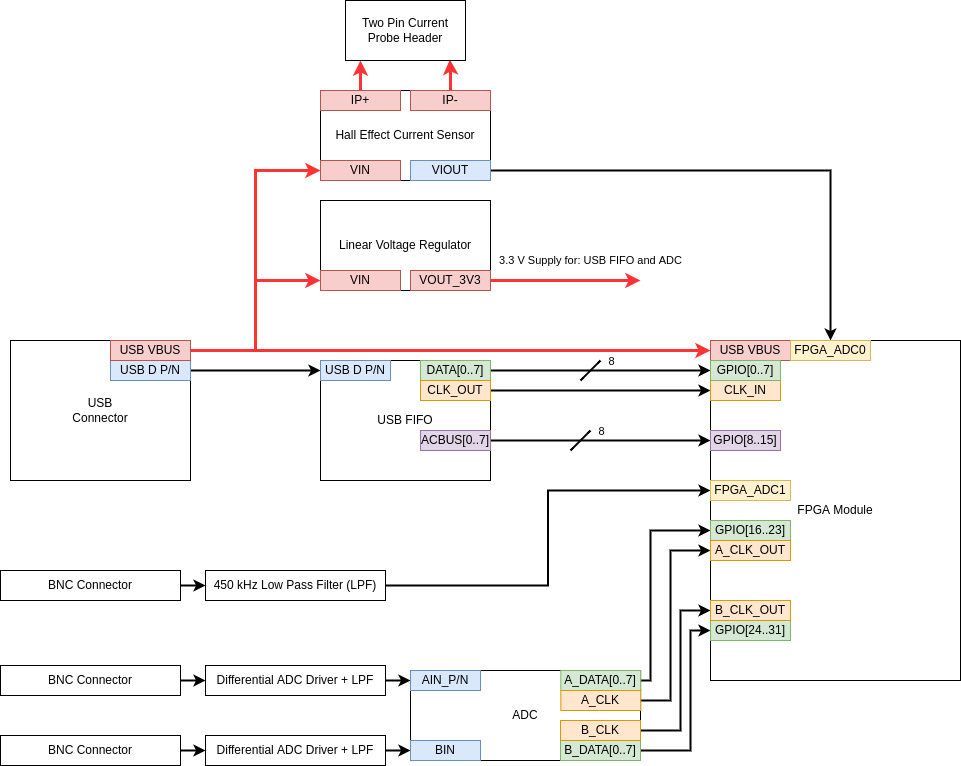
\includegraphics[width=16cm]{../../misc/TeachEE-System-Diagram.drawio.png}
            \caption{TeachEE PCB System Block Diagram}
            \label{fig:pcb-block-diagram}
        \end{figure}
        \begin{landscape}
        \section{Schematics}
        \label{appendix:schematic}
    \centering
    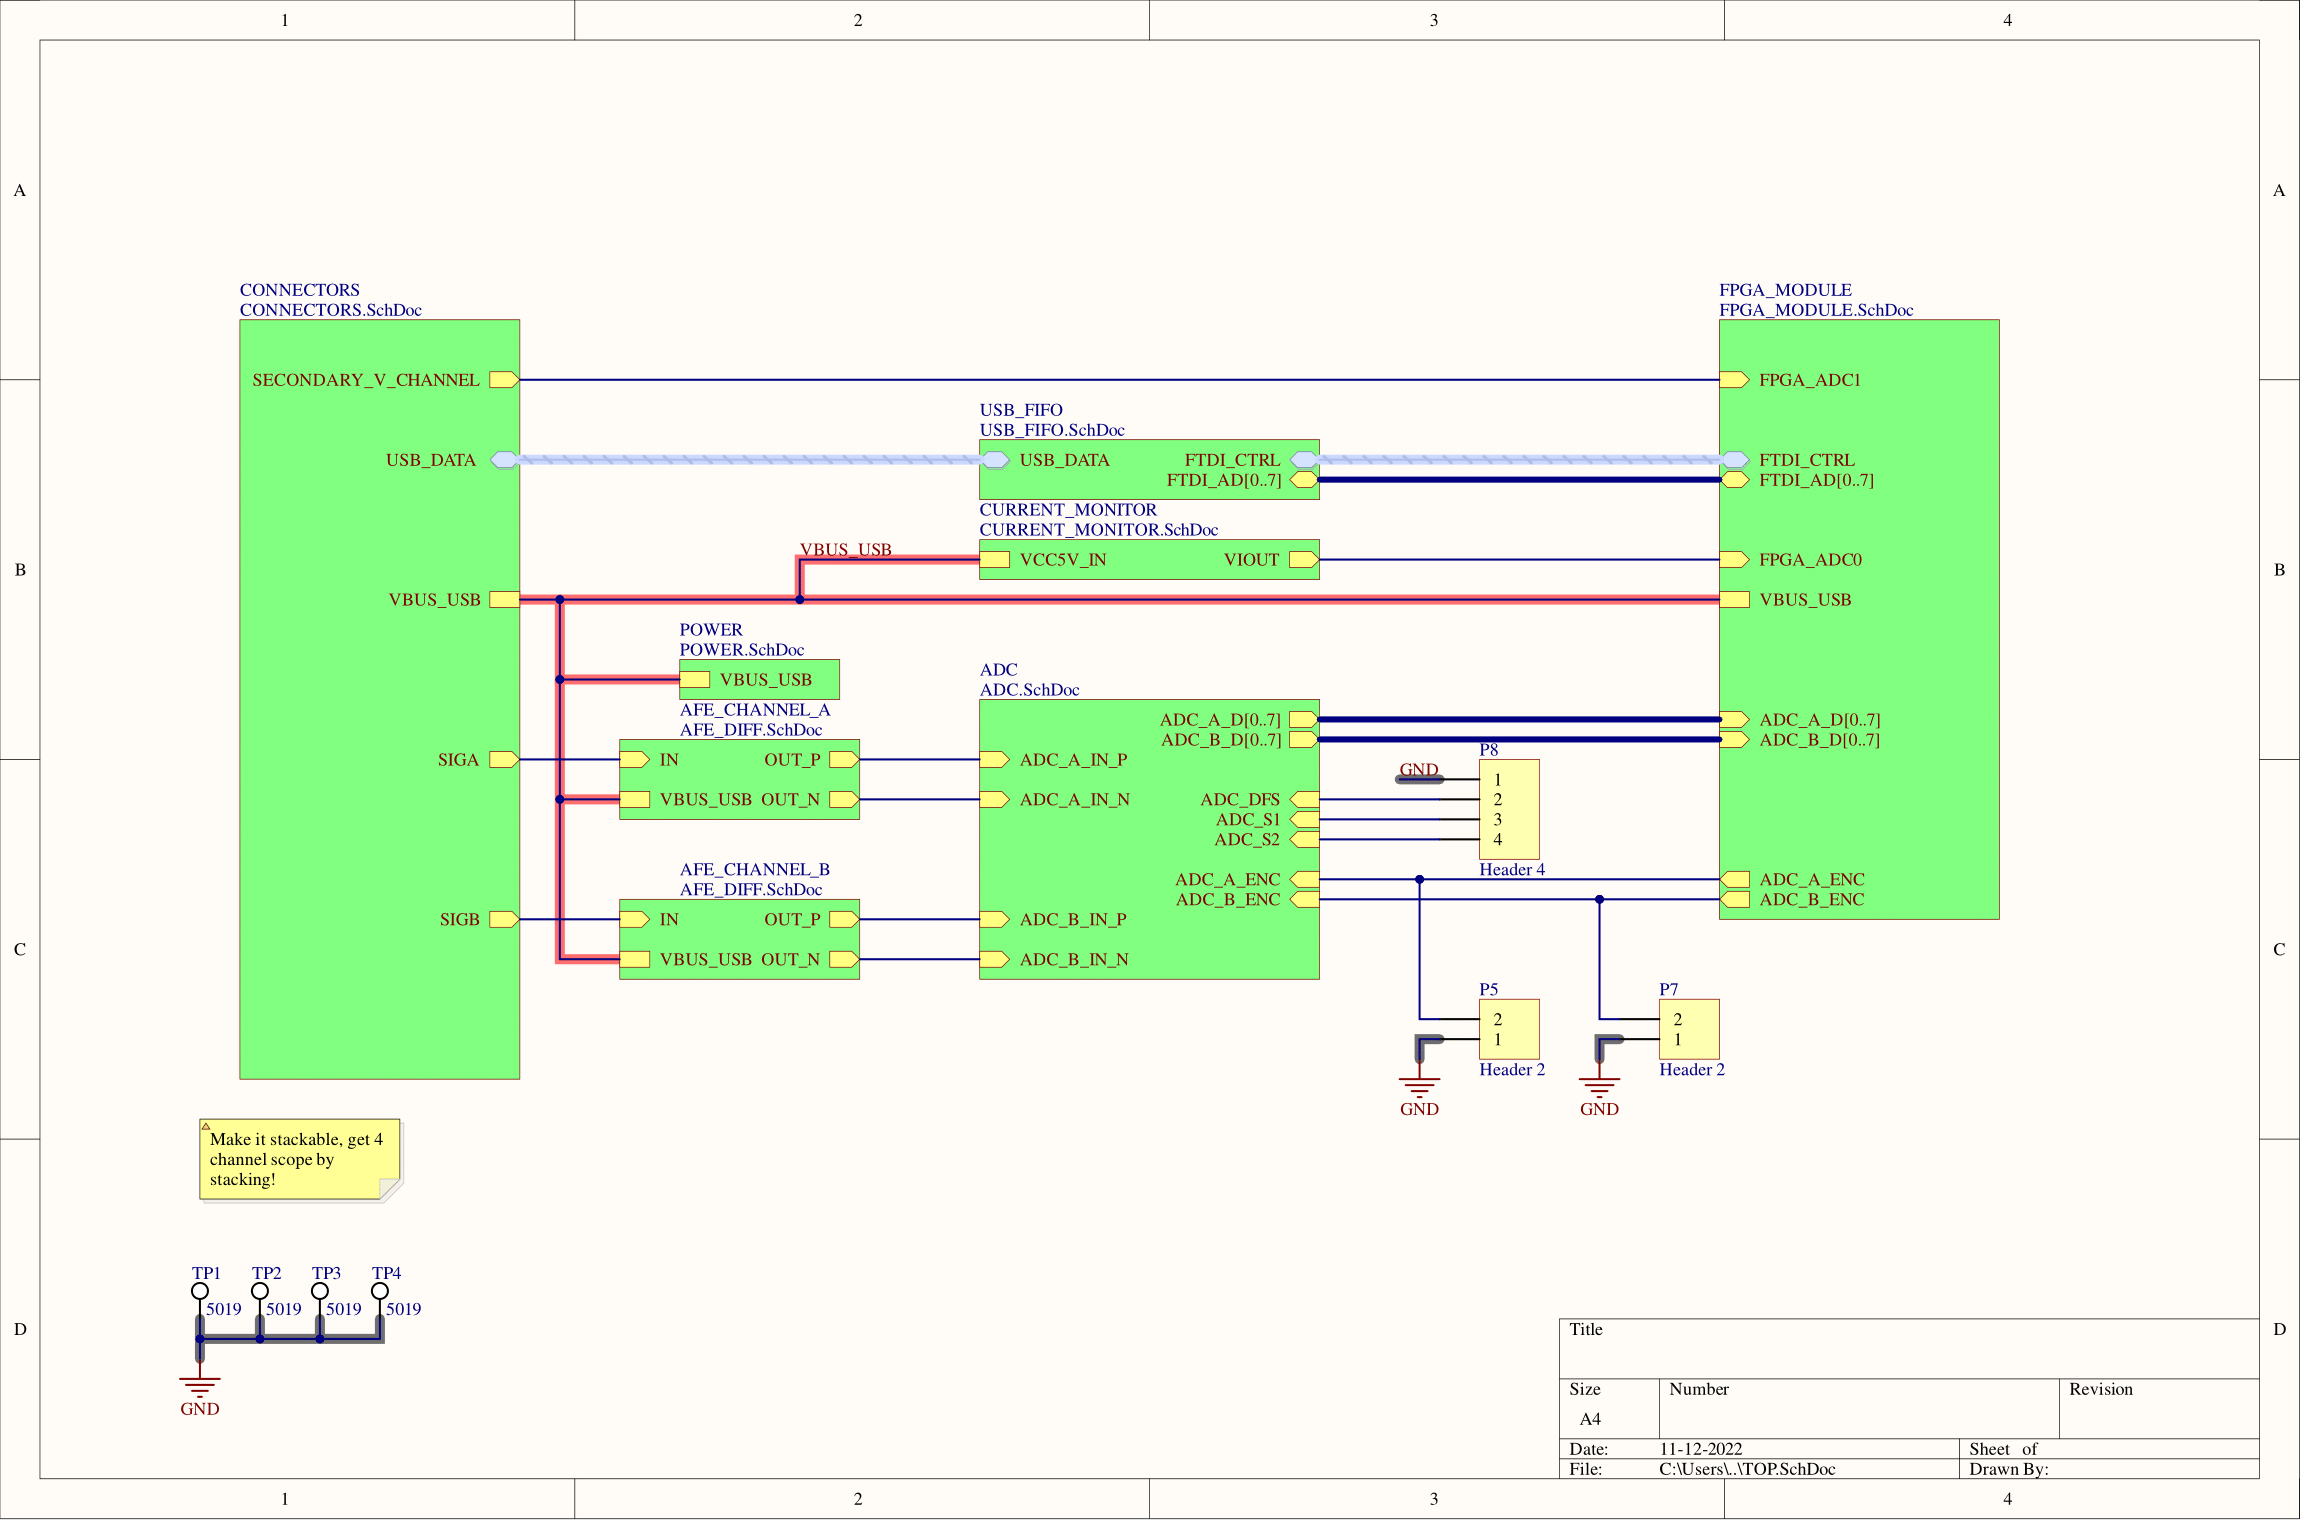
\includegraphics[height=15cm]{schematics/schematic1-1.png}
        \end{landscape}
    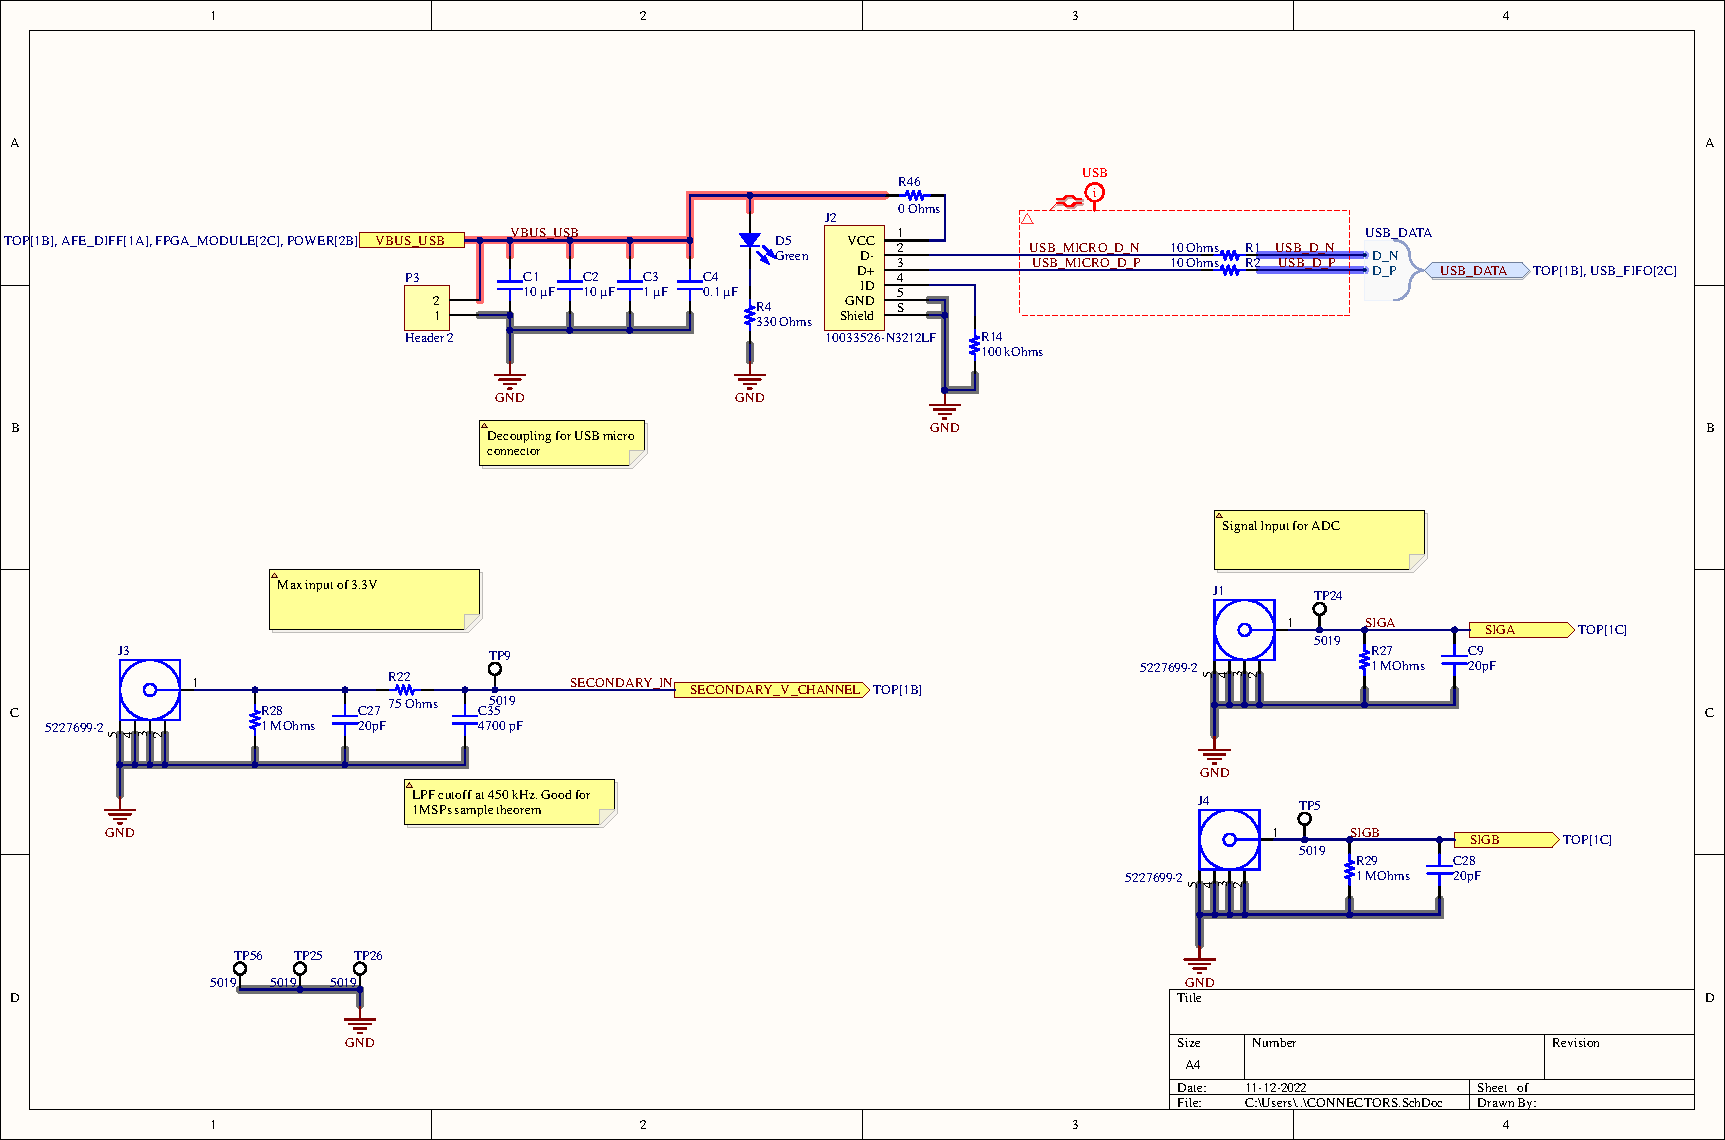
\includepdf[pages=-,landscape=true]{schematics/schematic2-8.pdf}

        \begin{landscape}
        \section{PCB Layout}
        \label{appendix:layout}
    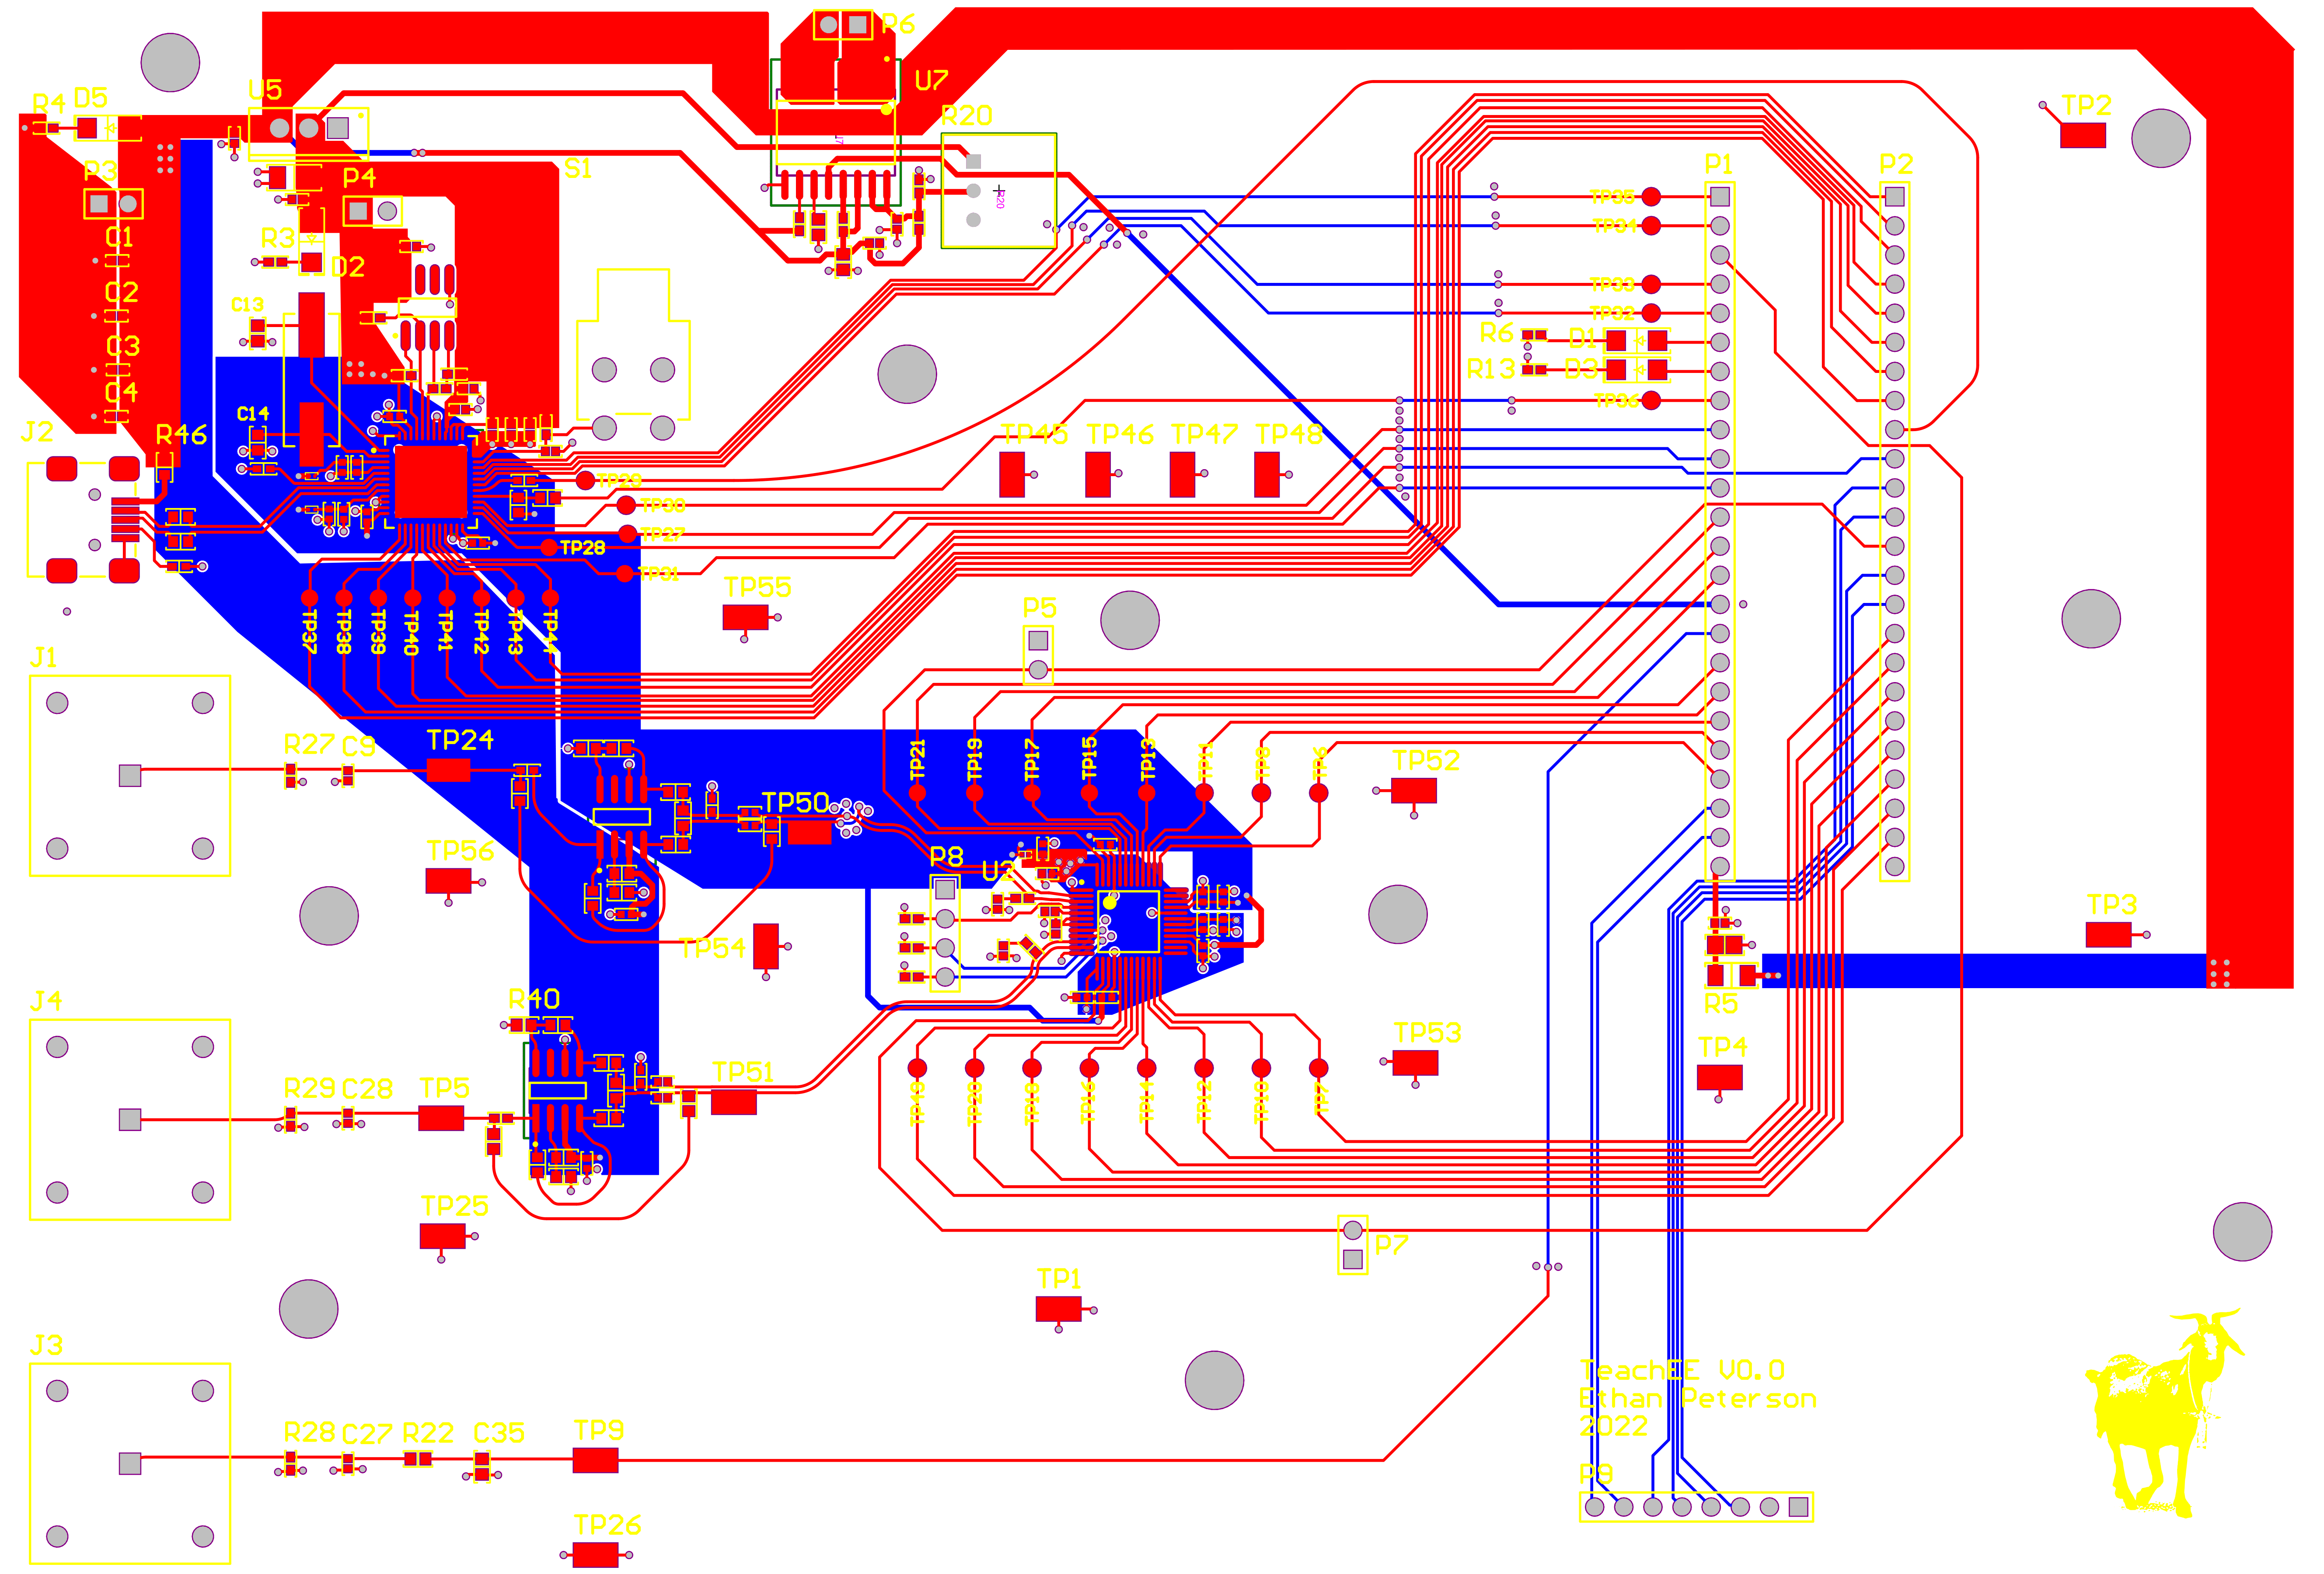
\includegraphics[height=15cm]{schematics/Layout.png}
        \end{landscape}

        \section{PCB Bill of Materials}
        \label{appendix:bom}
    \begin{table}[H]
    \begin{tabular}{p{1.7in}|p{0.3in}|p{0.8in}|p{0.7in}|p{0.7in}|p{1in}}
        \textbf{Designator} & \textbf{QTY} & \textbf{Description} & \textbf{Comment} & \textbf{Footprint} & \textbf{Part Number} \\ \hline 
        C1, C2, C37, C48 & 4 & CAP CER 10UF 10V X5R 0402 & 10 µF & CAP 0402\_1005 & CL05A106MP8NUB8 \\ \hline
        C3 & 1 & CAP CER 1UF 10V X7S 0402 & 1 µF & CAP 0402\_1005 & GRM155C71A105KE11D \\ \hline
        C4, C11, C16, C17, C18, C19, C20, C21, C22, C24, C26, C29, C30, C38, C39, C40, C41, C42, C43, C44, C45, C46, C47, C50\_AFE\_CHANNEL\_A, C50\_AFE\_CHANNEL\_B, C52\_AFE\_CHANNEL\_A, C52\_AFE\_CHANNEL\_B, C53\_AFE\_CHANNEL\_A, C53\_AFE\_CHANNEL\_B & 29 & CAP CER 0.1UF 50V X5R 0402 & 0.1 µF & CAP 0402\_1005 & CGA2B3X5R1H104M050BB \\ \hline
        C5, C12, C32, C34 & 4 & CAP CER 0.1UF 10V X7R 0402 & 0.1µF & CAP 0402\_1005 & 0402ZC104KAT2A \\ \hline
        C6 & 1 & CAP CER 10UF 16V X5R 1206 & 10 µF & CAP 1206\_3216 - 0.8MM & EMK316BJ106MD-T \\ \hline
        C7 & 1 & CAP CER 10UF 35V X6S 0805 & 10 µF & CAP 0805\_2012 & GRM21BC8YA106KE11L \\ \hline
        C8, C15, C23, C25 & 4 & CAP CER 4.7UF 16V X5R 0402 & 4.7 µF & CAP 0402\_1005 & CL05A475MO5NUNC \\ \hline
        C9, C27, C28 & 3 & CAP CER 20PF 25V NP0 0402 & 20pF & CAP 0402\_1005 & 04023U200JAT2A \\ \hline
    \end{tabular}
    \end{table}

    \newpage

    \begin{table}[H]
    \begin{tabular}{p{1.7in}|p{0.3in}|p{0.8in}|p{0.7in}|p{0.7in}|p{1in}}
        \textbf{Designator} & \textbf{QTY} & \textbf{Description} & \textbf{Comment} & \textbf{Footprint} & \textbf{Part Number} \\ \hline 
        C10 & 1 & CAP MLCC 0.01UF 100V X7R 0402 & 10000 pF & CAP 0402\_1005 & HMK105B7103KVHFE \\ \hline
        C13, C14 & 2 & CAP CER 36PF 100V NP0 0603 & 36pF & CAP 0603\_1608 & 06031A360JAT2A \\ \hline
        C31 & 1 & CAP CER 1UF 16V X7R 0603 & 1 µF & CAP 0603\_1608 & C0603C105K4RACAUTO \\ \hline
        C33, C35 & 2 & CAP CER 0603 4.7NF 16V X7R 10\% & 4700 pF & CAP 0603\_1608 & C0603C472K4RECAUTO \\ \hline
        C51\_AFE\_CHANNEL\_A, C51\_AFE\_CHANNEL\_B & 2 & CAP CER 15PF 25V C0G/NP0 0603 & 15 pF & CAP 0603\_1608 & C0603C150J3GACAUTO \\ \hline
        D1, D3 & 2 & LED SMD & Blue & LED 1206\_3216 BLUE & APTL3216QBC/D-01 \\ \hline
        D2, D5 & 2 & LED SMD & Green & LED 1206\_3216 GREEN & APTL3216ZGCK-01 \\ \hline
        FB1, FB2, FB3 & 3 & FERRITE BEAD 33 OHM 0201 1LN & 33 Ohms @ 100 MHz & FER 0201\_0603 & MMZ0603F330CT000 \\ \hline
        J1, J3, J4 & 3 & Jack BNC Connector, 1 Position, Height 16.26 mm, Tail Length 6.35 mm, -55 to 85 degC, RoHS, Tube & 5227699-2 & & 5227699-2 \\ \hline
        J2 & 1 & CONN RCPT MINI USB B 5POS SMD RA & & & 10033526-N3212LF \\ \hline
    \end{tabular}
    \end{table}
    \newpage
    \begin{table}[H]
        \begin{tabular}{p{1.7in}|p{0.3in}|p{0.8in}|p{0.7in}|p{0.7in}|p{1in}}
        \textbf{Designator} & \textbf{QTY} & \textbf{Description} & \textbf{Comment} & \textbf{Footprint} & \textbf{Part Number} \\ \hline 
        R1, R2 & 2 & RES SMD 10 OHM 0.1\% 1/10W 0603 & 10 Ohms & RES 0603\_1608 & CRT0603-BY-10R0ELF \\ \hline
        R3, R6, R13 & 3 & RES 220 OHM 1\% 1/8W 0402 & 220 Ohms & RES 0402\_1005 & CRGP0402F220R \\ \hline
        R4 & 1 & RES SMD 330 OHM 5\% 1/16W 0402 & 330 Ohms & RES 0402\_1005 & AC0402JR-07330RL \\ \hline
        R5 & 1 & 1206 40 AMP JUMPER & 0 Ohms & RES 1206\_3216 & JR1206X40E \\ \hline
        R7 & 1 & RES SMD 12K OHM 0.1\% 1/16W 0402 & 12 kOhms & RES 0402\_1005 & CPF0402B12KE1 \\ \hline
        R8, R9, R10, R11, R17, R18, R19, R21, R32, R33, R34 & 11 & RES 10K OHM 0.1\% 1/10W 0402 & 10 kOhms & RES 0402\_1005 & RP73PF1E10KBTD \\ \hline
        R12 & 1 & RES 1.8K OHM 1\% 1/16W 0402 & 1.8 kOhms & RES 0402\_1005 & RC0402FR-071K8L \\ \hline
        R14 & 1 & RES SMD 100K OHM 0.1\% 1/16W 0402 & 100 kOhms & RES 0402\_1005 & CPF0402B100KE \\ \hline
        R15, R46 & 2 & RES SMD 0 OHM JUMPER 1/2W 0603 & 0 Ohms & RES 0603\_1608 & 5110 \\ \hline
        R22 & 1 & RES SMD 75 OHM 1\% 1/10W 0603 & 75 Ohms & RES 0603\_1608 & AC0603FR-0775RL \\ \hline
        R26 & 1 & RES 24 OHM 1\% 1/16W 0402 & 24 Ohms & RES 0402\_1005 & RC0402FR-0724RL \\ \hline
        \end{tabular}
    \end{table}
    \newpage
    \begin{table}[H]
        \begin{tabular}{p{1.7in}|p{0.3in}|p{0.8in}|p{0.7in}|p{0.7in}|p{1in}}
        \textbf{Designator} & \textbf{QTY} & \textbf{Description} & \textbf{Comment} & \textbf{Footprint} & \textbf{Part Number} \\ \hline 
        R27, R28, R29 & 3 & RES 1M OHM 1\% 1/16W 0402 & 1 MOhms & RES 0402\_1005 & RMCF0402FT1M00 \\ \hline
        R36\_AFE\_CHANNEL\_A, R36\_AFE\_CHANNEL\_B & 2 & RES SMD 523 OHM 0.1\% 1/16W 0402 & 523 Ohms & RES 0402\_1005 & ERA-2ARB5230X \\ \hline
        R37\_AFE\_CHANNEL\_A, R37\_AFE\_CHANNEL\_B, R40\_AFE\_CHANNEL\_A, R40\_AFE\_CHANNEL\_B, R41\_AFE\_CHANNEL\_A, R41\_AFE\_CHANNEL\_B & 6 & RES SMD 500 OHM 0.05\% 1/10W 0603 & 500 Ohms & RES 0603\_1608 & TNPU0603500RAZEN00 \\ \hline
        R39\_AFE\_CHANNEL\_A, R39\_AFE\_CHANNEL\_B, R43\_AFE\_CHANNEL\_A, R43\_AFE\_CHANNEL\_B & 4 & RES 50 OHM 5\% 1/8W 0603 & 50 Ohms & RES 0603\_1608 & CH0603-50RJNTA \\ \hline
        R42\_AFE\_CHANNEL\_A, R42\_AFE\_CHANNEL\_B & 2 & RES SMD 4.02K OHM 1\% 1/10W 0603 & 4.02 kOhms & RES 0603\_1608 & AC0603FR-074K02L \\ \hline
        R44\_AFE\_CHANNEL\_A, R44\_AFE\_CHANNEL\_B & 2 & RES SMD 1K OHM 1\% 1/10W 0603 & 1 kOhms & RES 0603\_1608 & AA0603FR-071KL \\ \hline
        R45\_AFE\_CHANNEL\_A, R45\_AFE\_CHANNEL\_B & 2 & RES 25 OHM 0.1\% 1/20W 0402 & 25 Ohms & RES 0402\_1005 & FC0402E25R0BST0 \\ \hline
        S1 & 1 & SWITCH PUSH SPST-NO 0.4VA 28V & &  & AB11AH-HA \\ \hline
        TP1, TP2, TP3, TP4, TP5, TP9, TP24, TP25, TP26, TP45, TP46, TP47, TP48, TP50, TP51, TP52, TP53, TP54, TP55, TP56 & 20 & Test Point, 1 Position SMD, RoHS, Tape and Reel & 5019 & KSTN5019 & 5019 \\ \hline
        U1 & 1 & IC HS USB TO UART/FIFO 48QFN & FT232 & QFN-48 & FT232HQ-REEL \\ \hline
        \end{tabular}
    \end{table}
    \newpage
    \begin{table}[H]
        \begin{tabular}{p{1.7in}|p{0.3in}|p{0.8in}|p{0.7in}|p{0.7in}|p{1in}}
        \textbf{Designator} & \textbf{QTY} & \textbf{Description} & \textbf{Comment} & \textbf{Footprint} & \textbf{Part Number} \\ \hline 
        U2 & 1 & Dual 8-Bit AD Converter with Parallel Interface, 40MSPS, -40 to +85 degC, ST-48, Pb-Free, Tray &  & ST-48M & AD9288BSTZ-40 \\ \hline
        U3\_AFE\_CHANNEL\_A, U3\_AFE\_CHANNEL\_B & 2 & IC ADC DRIVER 8SOIC & AD8138 & R-8-IPC\_A & AD8138ARZ-R7 \\ \hline
        U5 & 1 & Fixed Low Drop Positive Voltage Regulator, 3.3V, 3-Pin TO-220 & LD1117 & TO220 & LD1117V33C \\ \hline
        U6 & 1 & 2K, 128x16-bit, 2.5V Microwire Serial EEPROM, 8-Pin SOIC 150mil, Commercial Temperature, Tape and Reel & 93LC56 & SOIC8 & 93LC56BT/SN \\ \hline
        U7 & 1 & CURRENT SENSOR & ACS720 &  & ACS720KLATR-15AB-T \\ \hline
        Y1 & 1 & CRYSTAL 12.0000MHZ 20PF SMD & 12 MHz & ABLS & ABLS-12.000MHZ-20-B-3-H-T \\ \hline
        \end{tabular}
    \end{table}

        \section{TeachEE Desktop App Screenshots}
        \label{appendix:screenshot}
    \begin{figure}[H]
        \centering
        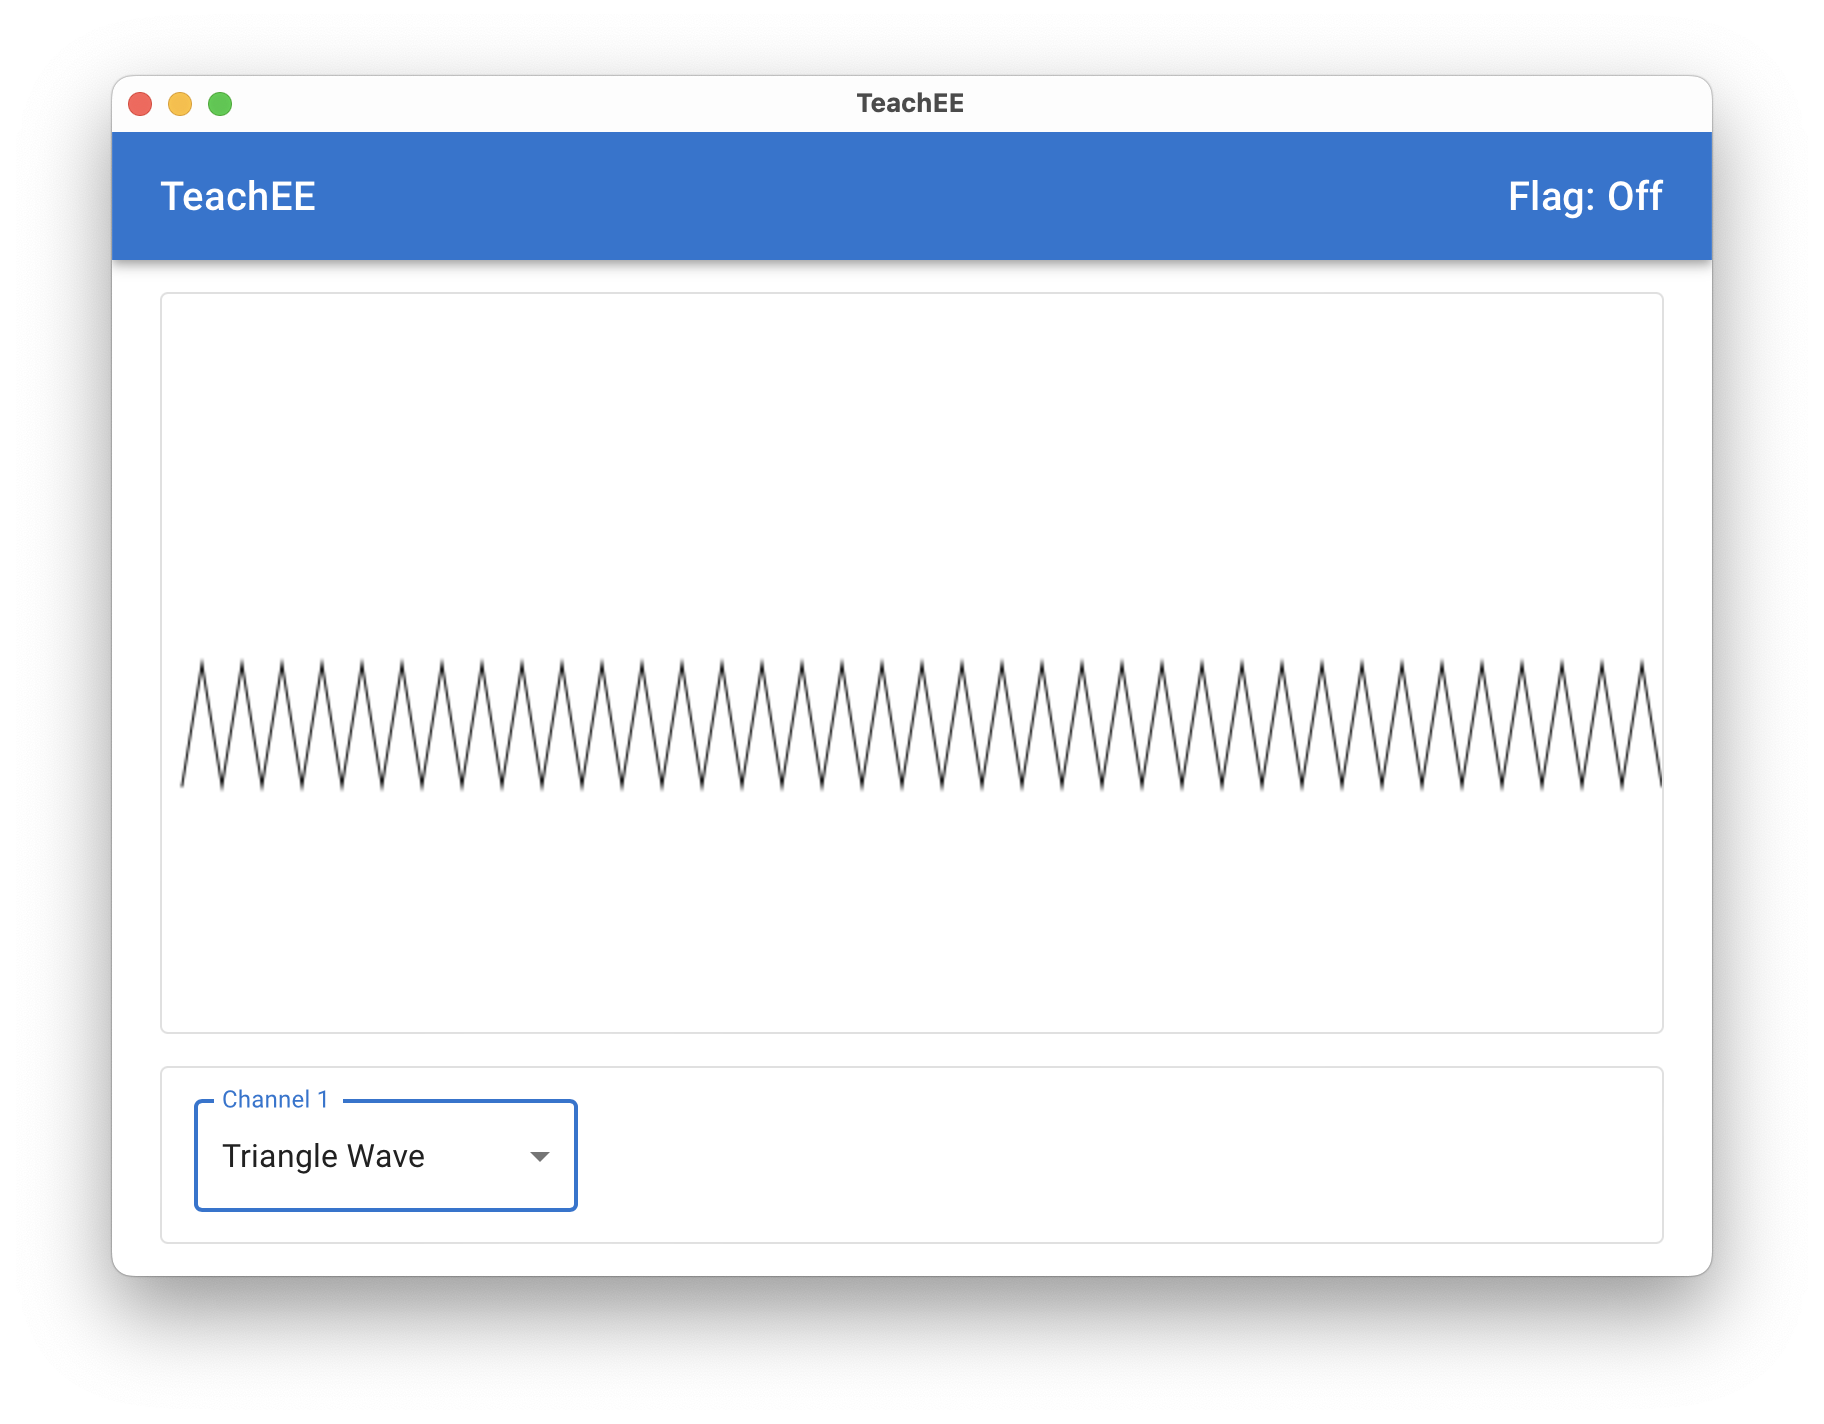
\includegraphics[width=\textwidth]{./schematics/sw-screenshot.png}
        \caption{TeachEE Desktop App Displaying a Triangle Wave}
    \end{figure}
        
    \end{appendices}
\end{document}
